% Paper A -- ACIIDS 2027 submission draft (Springer LNCS/LNAI).
% All numbers come from results.tex, generated by make_results.py from repository files.
\documentclass[runningheads]{llncs}
\usepackage[T1]{fontenc}
\usepackage{graphicx}
\usepackage{amsmath,amssymb}
\usepackage{booktabs}
\usepackage{xcolor}
\usepackage{tikz}
\usetikzlibrary{positioning,arrows.meta}
\usepackage[hidelinks]{hyperref}
\newif\ifpendshort
% \PENDING{key}: placeholder for a RIS-relevant-scope value that does not exist yet.
\newcommand{\PENDING}[1]{\textcolor{red}{\textbf{\ifpendshort P\else[#1]\fi}}}
% AUTO-GENERATED by make_results.py -- do not edit by hand.
% Sources: N=natural-scope leverage diagnostic (validation), G=ME-GA record / pair counts,
% P=production docs, V=v3 scope declaration, S=v3 search declaration, B=benchmark summary (--bench), PENDING=not yet produced.
\providecommand{\PENDING}[1]{\textcolor{red}{\textbf{[#1]}}}
\makeatletter
\newcommand{\res}[1]{\ifcsname res@#1\endcsname\csname res@#1\endcsname\else\PENDING{undefined:#1}\fi}
\expandafter\def\csname res@natApW64\endcsname{0.20}% N
\expandafter\def\csname res@natApH64\endcsname{0.21}% N
\expandafter\def\csname res@natApW128\endcsname{0.42}% N
\expandafter\def\csname res@natApH128\endcsname{0.21}% N
\expandafter\def\csname res@natApW256\endcsname{0.42}% N
\expandafter\def\csname res@natApH256\endcsname{0.45}% N
\expandafter\def\csname res@natFrames64\endcsname{864}% N
\expandafter\def\csname res@natZeroShare64\endcsname{49.1}% N
\expandafter\def\csname res@natZeroBoth64\endcsname{370}% N
\expandafter\def\csname res@natZeroTraj64\endcsname{23}% N
\expandafter\def\csname res@natTraj64\endcsname{54}% N
\expandafter\def\csname res@natOffMinusNoRis64\endcsname{+0.019}% N
\expandafter\def\csname res@natGainAllMean64\endcsname{0.026}% N
\expandafter\def\csname res@natGainAllMedian64\endcsname{0.000}% N
\expandafter\def\csname res@natGainNzMean64\endcsname{0.051}% N
\expandafter\def\csname res@natGainNzMedian64\endcsname{0.015}% N
\expandafter\def\csname res@natGainNzPninety64\endcsname{0.139}% N
\expandafter\def\csname res@natGainNzMax64\endcsname{0.674}% N
\expandafter\def\csname res@natGainGtOne64\endcsname{6.7}% N
\expandafter\def\csname res@natGainGtFive64\endcsname{0.6}% N
\expandafter\def\csname res@natRateOffMean64\endcsname{3.234}% N
\expandafter\def\csname res@natRateNoRisMean64\endcsname{3.215}% N
\expandafter\def\csname res@natRateBestMean64\endcsname{3.260}% N
\expandafter\def\csname res@natRateOnMean64\endcsname{3.181}% N
\expandafter\def\csname res@natRateBestOwnMean64\endcsname{3.253}% N
\expandafter\def\csname res@natIN64\endcsname{$-$6.9}% N
\expandafter\def\csname res@natPrecErr64\endcsname{0}% N
\expandafter\def\csname res@natRisDirBlkLos64\endcsname{$-$55.6}% N
\expandafter\def\csname res@natBoundBlkLos64\endcsname{$-$41.6}% N
\expandafter\def\csname res@natUFBlkLos64\endcsname{340}% N
\expandafter\def\csname res@natRisDirRefLos64\endcsname{$-$55.7}% N
\expandafter\def\csname res@natBoundRefLos64\endcsname{$-$43.2}% N
\expandafter\def\csname res@natUFRefLos64\endcsname{350}% N
\expandafter\def\csname res@natRisDirLosLos64\endcsname{$-$59.2}% N
\expandafter\def\csname res@natBoundLosLos64\endcsname{$-$40.8}% N
\expandafter\def\csname res@natUFLosLos64\endcsname{969}% N
\expandafter\def\csname res@natRisDirBlkRef64\endcsname{+19.6}% N
\expandafter\def\csname res@natBoundBlkRef64\endcsname{$-$41.9}% N
\expandafter\def\csname res@natUFBlkRef64\endcsname{18}% N
\expandafter\def\csname res@natHrNLosLos64\endcsname{136}% N
\expandafter\def\csname res@natHrMedLosLos64\endcsname{0.027}% N
\expandafter\def\csname res@natHrGtLosLos64\endcsname{17}% N
\expandafter\def\csname res@natHrNBlkLos64\endcsname{115}% N
\expandafter\def\csname res@natHrMedBlkLos64\endcsname{0.023}% N
\expandafter\def\csname res@natHrGtBlkLos64\endcsname{24}% N
\expandafter\def\csname res@natZeroMunich64\endcsname{56}% N
\expandafter\def\csname res@natZeroRotterdam64\endcsname{28}% N
\expandafter\def\csname res@natZeroMaastricht64\endcsname{64}% N
\expandafter\def\csname res@natFrames128\endcsname{864}% N
\expandafter\def\csname res@natZeroShare128\endcsname{49.1}% N
\expandafter\def\csname res@natZeroBoth128\endcsname{376}% N
\expandafter\def\csname res@natZeroTraj128\endcsname{23}% N
\expandafter\def\csname res@natTraj128\endcsname{54}% N
\expandafter\def\csname res@natOffMinusNoRis128\endcsname{+0.025}% N
\expandafter\def\csname res@natGainAllMean128\endcsname{0.035}% N
\expandafter\def\csname res@natGainAllMedian128\endcsname{0.000}% N
\expandafter\def\csname res@natGainNzMean128\endcsname{0.069}% N
\expandafter\def\csname res@natGainNzMedian128\endcsname{0.022}% N
\expandafter\def\csname res@natGainNzPninety128\endcsname{0.170}% N
\expandafter\def\csname res@natGainNzMax128\endcsname{0.831}% N
\expandafter\def\csname res@natGainGtOne128\endcsname{10.1}% N
\expandafter\def\csname res@natGainGtFive128\endcsname{1.2}% N
\expandafter\def\csname res@natRateOffMean128\endcsname{3.315}% N
\expandafter\def\csname res@natRateNoRisMean128\endcsname{3.290}% N
\expandafter\def\csname res@natRateBestMean128\endcsname{3.350}% N
\expandafter\def\csname res@natRateOnMean128\endcsname{3.240}% N
\expandafter\def\csname res@natRateBestOwnMean128\endcsname{3.344}% N
\expandafter\def\csname res@natIN128\endcsname{$-$2.6}% N
\expandafter\def\csname res@natPrecErr128\endcsname{0}% N
\expandafter\def\csname res@natRisDirBlkLos128\endcsname{$-$52.8}% N
\expandafter\def\csname res@natBoundBlkLos128\endcsname{$-$36.0}% N
\expandafter\def\csname res@natUFBlkLos128\endcsname{333}% N
\expandafter\def\csname res@natRisDirRefLos128\endcsname{$-$49.6}% N
\expandafter\def\csname res@natBoundRefLos128\endcsname{$-$36.5}% N
\expandafter\def\csname res@natUFRefLos128\endcsname{358}% N
\expandafter\def\csname res@natRisDirLosLos128\endcsname{$-$57.6}% N
\expandafter\def\csname res@natBoundLosLos128\endcsname{$-$34.2}% N
\expandafter\def\csname res@natUFLosLos128\endcsname{972}% N
\expandafter\def\csname res@natRisDirBlkRef128\endcsname{+19.4}% N
\expandafter\def\csname res@natBoundBlkRef128\endcsname{$-$35.2}% N
\expandafter\def\csname res@natUFBlkRef128\endcsname{18}% N
\expandafter\def\csname res@natHrNLosLos128\endcsname{118}% N
\expandafter\def\csname res@natHrMedLosLos128\endcsname{0.050}% N
\expandafter\def\csname res@natHrGtLosLos128\endcsname{33}% N
\expandafter\def\csname res@natHrNBlkLos128\endcsname{104}% N
\expandafter\def\csname res@natHrMedBlkLos128\endcsname{0.029}% N
\expandafter\def\csname res@natHrGtBlkLos128\endcsname{27}% N
\expandafter\def\csname res@natZeroMunich128\endcsname{56}% N
\expandafter\def\csname res@natZeroRotterdam128\endcsname{28}% N
\expandafter\def\csname res@natZeroMaastricht128\endcsname{64}% N
\expandafter\def\csname res@natFrames256\endcsname{864}% N
\expandafter\def\csname res@natZeroShare256\endcsname{49.7}% N
\expandafter\def\csname res@natZeroBoth256\endcsname{381}% N
\expandafter\def\csname res@natZeroTraj256\endcsname{23}% N
\expandafter\def\csname res@natTraj256\endcsname{54}% N
\expandafter\def\csname res@natOffMinusNoRis256\endcsname{+0.043}% N
\expandafter\def\csname res@natGainAllMean256\endcsname{0.060}% N
\expandafter\def\csname res@natGainAllMedian256\endcsname{0.000}% N
\expandafter\def\csname res@natGainNzMean256\endcsname{0.120}% N
\expandafter\def\csname res@natGainNzMedian256\endcsname{0.045}% N
\expandafter\def\csname res@natGainNzPninety256\endcsname{0.292}% N
\expandafter\def\csname res@natGainNzMax256\endcsname{1.488}% N
\expandafter\def\csname res@natGainGtOne256\endcsname{16.3}% N
\expandafter\def\csname res@natGainGtFive256\endcsname{2.8}% N
\expandafter\def\csname res@natRateOffMean256\endcsname{3.242}% N
\expandafter\def\csname res@natRateNoRisMean256\endcsname{3.199}% N
\expandafter\def\csname res@natRateBestMean256\endcsname{3.303}% N
\expandafter\def\csname res@natRateOnMean256\endcsname{3.137}% N
\expandafter\def\csname res@natRateBestOwnMean256\endcsname{3.293}% N
\expandafter\def\csname res@natIN256\endcsname{$-$7.2}% N
\expandafter\def\csname res@natPrecErr256\endcsname{0}% N
\expandafter\def\csname res@natRisDirBlkLos256\endcsname{$-$40.9}% N
\expandafter\def\csname res@natBoundBlkLos256\endcsname{$-$29.4}% N
\expandafter\def\csname res@natUFBlkLos256\endcsname{345}% N
\expandafter\def\csname res@natRisDirRefLos256\endcsname{$-$43.8}% N
\expandafter\def\csname res@natBoundRefLos256\endcsname{$-$29.2}% N
\expandafter\def\csname res@natUFRefLos256\endcsname{346}% N
\expandafter\def\csname res@natRisDirLosLos256\endcsname{$-$56.0}% N
\expandafter\def\csname res@natBoundLosLos256\endcsname{$-$27.6}% N
\expandafter\def\csname res@natUFLosLos256\endcsname{972}% N
\expandafter\def\csname res@natRisDirBlkRef256\endcsname{+19.6}% N
\expandafter\def\csname res@natBoundBlkRef256\endcsname{$-$28.6}% N
\expandafter\def\csname res@natUFBlkRef256\endcsname{18}% N
\expandafter\def\csname res@natHrNLosLos256\endcsname{110}% N
\expandafter\def\csname res@natHrMedLosLos256\endcsname{0.125}% N
\expandafter\def\csname res@natHrGtLosLos256\endcsname{55}% N
\expandafter\def\csname res@natHrNBlkLos256\endcsname{140}% N
\expandafter\def\csname res@natHrMedBlkLos256\endcsname{0.047}% N
\expandafter\def\csname res@natHrGtBlkLos256\endcsname{35}% N
\expandafter\def\csname res@natZeroMunich256\endcsname{56}% N
\expandafter\def\csname res@natZeroRotterdam256\endcsname{28}% N
\expandafter\def\csname res@natZeroMaastricht256\endcsname{65}% N
\expandafter\def\csname res@natFramesTotal\endcsname{2,592}% N
\expandafter\def\csname res@freqGHz\endcsname{5.53}% N
\expandafter\def\csname res@lambdaMm\endcsname{54.2}% N
\expandafter\def\csname res@boundXtenDb\endcsname{11}% N
\expandafter\def\csname res@natDbsrisMedian\endcsname{112}% N
\expandafter\def\csname res@natDbsrisMax\endcsname{150}% N
\expandafter\def\csname res@natDrisUserLo\endcsname{63}% N
\expandafter\def\csname res@natDrisUserHi\endcsname{136}% N
\expandafter\def\csname res@prodTrajPerMap\endcsname{120}% P
\expandafter\def\csname res@prodTraj\endcsname{360}% P
\expandafter\def\csname res@prodFramesPerTraj\endcsname{16}% P
\expandafter\def\csname res@prodFrames\endcsname{5,760}% P
\expandafter\def\csname res@prodArrayFrames\endcsname{17,280}% P
\expandafter\def\csname res@prodValTraj\endcsname{54}% P
\expandafter\def\csname res@siteDminNat\endcsname{20}% P
\expandafter\def\csname res@siteDmaxNat\endcsname{150}% P
\expandafter\def\csname res@negSlotProb\endcsname{0.15}% P
\expandafter\def\csname res@rtSamples\endcsname{10,000}% P
\expandafter\def\csname res@rtDepth\endcsname{2}% P
\expandafter\def\csname res@openGapPct\endcsname{4.7}% P
\expandafter\def\csname res@megaPop\endcsname{100}% G
\expandafter\def\csname res@megaIter\endcsname{100}% G
\expandafter\def\csname res@megaDecisions\endcsname{24}% G
\expandafter\def\csname res@megaSensItems\endcsname{9}% G
\expandafter\def\csname res@nPairsSixtyFour\endcsname{2,016}% G
\expandafter\def\csname res@nPairsOneTwentyEight\endcsname{8,128}% G
\expandafter\def\csname res@nPairsTwoFiftySix\endcsname{32,640}% G
\expandafter\def\csname res@megaWoodM\endcsname{24}% G
\expandafter\def\csname res@megaWoodMin\endcsname{12}% G
\expandafter\def\csname res@nsgaPop\endcsname{20}% G
\expandafter\def\csname res@nsgaPc\endcsname{0.9}% G
\expandafter\def\csname res@nsgaGridP\endcsname{20/50/100}% G
\expandafter\def\csname res@nsgaGridPc\endcsname{0.7/0.9}% G
\expandafter\def\csname res@nsgaGridN\endcsname{6}% G
\expandafter\def\csname res@vMap\endcsname{Rotterdam}% V
\expandafter\def\csname res@vTraj\endcsname{120}% V
\expandafter\def\csname res@vFrames\endcsname{16}% V
\expandafter\def\csname res@vTrainTraj\endcsname{84}% V
\expandafter\def\csname res@vValTraj\endcsname{18}% V
\expandafter\def\csname res@vTestTraj\endcsname{18}% V
\expandafter\def\csname res@vDmin\endcsname{5}% V
\expandafter\def\csname res@vDmax\endcsname{20}% V
\expandafter\def\csname res@vDOneMin\endcsname{7.8}% V
\expandafter\def\csname res@vDOneMed\endcsname{13.7}% V
\expandafter\def\csname res@vDOneMax\endcsname{18.7}% V
\expandafter\def\csname res@vSites\endcsname{4}% V
\expandafter\def\csname res@vDTwoLo\endcsname{26.7}% V
\expandafter\def\csname res@vDTwoMed\endcsname{32.3}% V
\expandafter\def\csname res@vDTwoHi\endcsname{36.4}% V
\expandafter\def\csname res@vRadius\endcsname{40}% V
\expandafter\def\csname res@vAngle\endcsname{80}% V
\expandafter\def\csname res@vServedUF\endcsname{4,800}% V
\expandafter\def\csname res@vSamples\endcsname{10^{6}}% V
\expandafter\def\csname res@vPathCap\endcsname{2\times10^{6}}% V
\expandafter\def\csname res@vDepth\endcsname{2}% V
\expandafter\def\csname res@vUnitsOk\endcsname{357}% V
\expandafter\def\csname res@vUnits\endcsname{360}% V
\expandafter\def\csname res@vIncluded\endcsname{119}% V
\expandafter\def\csname res@vGainMed64\endcsname{0.302}% V
\expandafter\def\csname res@vGainMed128\endcsname{0.418}% V
\expandafter\def\csname res@vGainMed256\endcsname{0.782}% V
\expandafter\def\csname res@vGainMean64\endcsname{0.450}% V
\expandafter\def\csname res@vGainPninety64\endcsname{1.089}% V
\expandafter\def\csname res@vGainMean128\endcsname{0.534}% V
\expandafter\def\csname res@vGainPninety128\endcsname{1.379}% V
\expandafter\def\csname res@vGainMean256\endcsname{1.097}% V
\expandafter\def\csname res@vGainPninety256\endcsname{2.760}% V
\expandafter\def\csname res@vPathless\endcsname{0.0}% V
\expandafter\def\csname res@vSeeds\endcsname{10}% S
\expandafter\def\csname res@vBoot\endcsname{10,000}% S
\expandafter\def\csname res@vFamily\endcsname{five}% S
\expandafter\def\csname res@vMaxMiss\endcsname{0.5}% S
\expandafter\def\csname res@vRateGreedyFive64\endcsname{\PENDING{vRateGreedyFive64}}% PENDING
\expandafter\def\csname res@vRateGreedyTen64\endcsname{\PENDING{vRateGreedyTen64}}% PENDING
\expandafter\def\csname res@vRateGreedyFifty64\endcsname{\PENDING{vRateGreedyFifty64}}% PENDING
\expandafter\def\csname res@vRateGreedyHundred64\endcsname{\PENDING{vRateGreedyHundred64}}% PENDING
\expandafter\def\csname res@vLatGreedy64\endcsname{\PENDING{vLatGreedy64}}% PENDING
\expandafter\def\csname res@vLatPGreedy64\endcsname{\PENDING{vLatPGreedy64}}% PENDING
\expandafter\def\csname res@vEvalsGreedy64\endcsname{\PENDING{vEvalsGreedy64}}% PENDING
\expandafter\def\csname res@vMissGreedy64\endcsname{\PENDING{vMissGreedy64}}% PENDING
\expandafter\def\csname res@vRatePairFive64\endcsname{\PENDING{vRatePairFive64}}% PENDING
\expandafter\def\csname res@vRatePairTen64\endcsname{\PENDING{vRatePairTen64}}% PENDING
\expandafter\def\csname res@vRatePairFifty64\endcsname{\PENDING{vRatePairFifty64}}% PENDING
\expandafter\def\csname res@vRatePairHundred64\endcsname{\PENDING{vRatePairHundred64}}% PENDING
\expandafter\def\csname res@vLatPair64\endcsname{\PENDING{vLatPair64}}% PENDING
\expandafter\def\csname res@vLatPPair64\endcsname{\PENDING{vLatPPair64}}% PENDING
\expandafter\def\csname res@vEvalsPair64\endcsname{\PENDING{vEvalsPair64}}% PENDING
\expandafter\def\csname res@vMissPair64\endcsname{\PENDING{vMissPair64}}% PENDING
\expandafter\def\csname res@vRateBthreeFive64\endcsname{\PENDING{vRateBthreeFive64}}% PENDING
\expandafter\def\csname res@vRateBthreeTen64\endcsname{\PENDING{vRateBthreeTen64}}% PENDING
\expandafter\def\csname res@vRateBthreeFifty64\endcsname{\PENDING{vRateBthreeFifty64}}% PENDING
\expandafter\def\csname res@vRateBthreeHundred64\endcsname{\PENDING{vRateBthreeHundred64}}% PENDING
\expandafter\def\csname res@vLatBthree64\endcsname{\PENDING{vLatBthree64}}% PENDING
\expandafter\def\csname res@vLatPBthree64\endcsname{\PENDING{vLatPBthree64}}% PENDING
\expandafter\def\csname res@vEvalsBthree64\endcsname{\PENDING{vEvalsBthree64}}% PENDING
\expandafter\def\csname res@vMissBthree64\endcsname{\PENDING{vMissBthree64}}% PENDING
\expandafter\def\csname res@vRateBfiveFive64\endcsname{\PENDING{vRateBfiveFive64}}% PENDING
\expandafter\def\csname res@vRateBfiveTen64\endcsname{\PENDING{vRateBfiveTen64}}% PENDING
\expandafter\def\csname res@vRateBfiveFifty64\endcsname{\PENDING{vRateBfiveFifty64}}% PENDING
\expandafter\def\csname res@vRateBfiveHundred64\endcsname{\PENDING{vRateBfiveHundred64}}% PENDING
\expandafter\def\csname res@vLatBfive64\endcsname{\PENDING{vLatBfive64}}% PENDING
\expandafter\def\csname res@vLatPBfive64\endcsname{\PENDING{vLatPBfive64}}% PENDING
\expandafter\def\csname res@vEvalsBfive64\endcsname{\PENDING{vEvalsBfive64}}% PENDING
\expandafter\def\csname res@vMissBfive64\endcsname{\PENDING{vMissBfive64}}% PENDING
\expandafter\def\csname res@vRateBtsFive64\endcsname{\PENDING{vRateBtsFive64}}% PENDING
\expandafter\def\csname res@vRateBtsTen64\endcsname{\PENDING{vRateBtsTen64}}% PENDING
\expandafter\def\csname res@vRateBtsFifty64\endcsname{\PENDING{vRateBtsFifty64}}% PENDING
\expandafter\def\csname res@vRateBtsHundred64\endcsname{\PENDING{vRateBtsHundred64}}% PENDING
\expandafter\def\csname res@vLatBts64\endcsname{\PENDING{vLatBts64}}% PENDING
\expandafter\def\csname res@vLatPBts64\endcsname{\PENDING{vLatPBts64}}% PENDING
\expandafter\def\csname res@vEvalsBts64\endcsname{\PENDING{vEvalsBts64}}% PENDING
\expandafter\def\csname res@vMissBts64\endcsname{\PENDING{vMissBts64}}% PENDING
\expandafter\def\csname res@vRateMegaFive64\endcsname{\PENDING{vRateMegaFive64}}% PENDING
\expandafter\def\csname res@vRateMegaTen64\endcsname{\PENDING{vRateMegaTen64}}% PENDING
\expandafter\def\csname res@vRateMegaFifty64\endcsname{\PENDING{vRateMegaFifty64}}% PENDING
\expandafter\def\csname res@vRateMegaHundred64\endcsname{\PENDING{vRateMegaHundred64}}% PENDING
\expandafter\def\csname res@vLatMega64\endcsname{\PENDING{vLatMega64}}% PENDING
\expandafter\def\csname res@vLatPMega64\endcsname{\PENDING{vLatPMega64}}% PENDING
\expandafter\def\csname res@vEvalsMega64\endcsname{\PENDING{vEvalsMega64}}% PENDING
\expandafter\def\csname res@vMissMega64\endcsname{\PENDING{vMissMega64}}% PENDING
\expandafter\def\csname res@vRateNsgaFive64\endcsname{\PENDING{vRateNsgaFive64}}% PENDING
\expandafter\def\csname res@vRateNsgaTen64\endcsname{\PENDING{vRateNsgaTen64}}% PENDING
\expandafter\def\csname res@vRateNsgaFifty64\endcsname{\PENDING{vRateNsgaFifty64}}% PENDING
\expandafter\def\csname res@vRateNsgaHundred64\endcsname{\PENDING{vRateNsgaHundred64}}% PENDING
\expandafter\def\csname res@vLatNsga64\endcsname{\PENDING{vLatNsga64}}% PENDING
\expandafter\def\csname res@vLatPNsga64\endcsname{\PENDING{vLatPNsga64}}% PENDING
\expandafter\def\csname res@vEvalsNsga64\endcsname{\PENDING{vEvalsNsga64}}% PENDING
\expandafter\def\csname res@vMissNsga64\endcsname{\PENDING{vMissNsga64}}% PENDING
\expandafter\def\csname res@vHOne64\endcsname{\PENDING{vHOne64}}% PENDING
\expandafter\def\csname res@vHOneVerdict64\endcsname{\PENDING{vHOneVerdict64}}% PENDING
\expandafter\def\csname res@vHTwo64\endcsname{\PENDING{vHTwo64}}% PENDING
\expandafter\def\csname res@vHTwoVerdict64\endcsname{\PENDING{vHTwoVerdict64}}% PENDING
\expandafter\def\csname res@vHFive64\endcsname{\PENDING{vHFive64}}% PENDING
\expandafter\def\csname res@vHFiveVerdict64\endcsname{\PENDING{vHFiveVerdict64}}% PENDING
\expandafter\def\csname res@vRateGreedyFive128\endcsname{\PENDING{vRateGreedyFive128}}% PENDING
\expandafter\def\csname res@vRateGreedyTen128\endcsname{\PENDING{vRateGreedyTen128}}% PENDING
\expandafter\def\csname res@vRateGreedyFifty128\endcsname{\PENDING{vRateGreedyFifty128}}% PENDING
\expandafter\def\csname res@vRateGreedyHundred128\endcsname{\PENDING{vRateGreedyHundred128}}% PENDING
\expandafter\def\csname res@vLatGreedy128\endcsname{\PENDING{vLatGreedy128}}% PENDING
\expandafter\def\csname res@vLatPGreedy128\endcsname{\PENDING{vLatPGreedy128}}% PENDING
\expandafter\def\csname res@vEvalsGreedy128\endcsname{\PENDING{vEvalsGreedy128}}% PENDING
\expandafter\def\csname res@vMissGreedy128\endcsname{\PENDING{vMissGreedy128}}% PENDING
\expandafter\def\csname res@vRatePairFive128\endcsname{\PENDING{vRatePairFive128}}% PENDING
\expandafter\def\csname res@vRatePairTen128\endcsname{\PENDING{vRatePairTen128}}% PENDING
\expandafter\def\csname res@vRatePairFifty128\endcsname{\PENDING{vRatePairFifty128}}% PENDING
\expandafter\def\csname res@vRatePairHundred128\endcsname{\PENDING{vRatePairHundred128}}% PENDING
\expandafter\def\csname res@vLatPair128\endcsname{\PENDING{vLatPair128}}% PENDING
\expandafter\def\csname res@vLatPPair128\endcsname{\PENDING{vLatPPair128}}% PENDING
\expandafter\def\csname res@vEvalsPair128\endcsname{\PENDING{vEvalsPair128}}% PENDING
\expandafter\def\csname res@vMissPair128\endcsname{\PENDING{vMissPair128}}% PENDING
\expandafter\def\csname res@vRateBthreeFive128\endcsname{\PENDING{vRateBthreeFive128}}% PENDING
\expandafter\def\csname res@vRateBthreeTen128\endcsname{\PENDING{vRateBthreeTen128}}% PENDING
\expandafter\def\csname res@vRateBthreeFifty128\endcsname{\PENDING{vRateBthreeFifty128}}% PENDING
\expandafter\def\csname res@vRateBthreeHundred128\endcsname{\PENDING{vRateBthreeHundred128}}% PENDING
\expandafter\def\csname res@vLatBthree128\endcsname{\PENDING{vLatBthree128}}% PENDING
\expandafter\def\csname res@vLatPBthree128\endcsname{\PENDING{vLatPBthree128}}% PENDING
\expandafter\def\csname res@vEvalsBthree128\endcsname{\PENDING{vEvalsBthree128}}% PENDING
\expandafter\def\csname res@vMissBthree128\endcsname{\PENDING{vMissBthree128}}% PENDING
\expandafter\def\csname res@vRateBfiveFive128\endcsname{\PENDING{vRateBfiveFive128}}% PENDING
\expandafter\def\csname res@vRateBfiveTen128\endcsname{\PENDING{vRateBfiveTen128}}% PENDING
\expandafter\def\csname res@vRateBfiveFifty128\endcsname{\PENDING{vRateBfiveFifty128}}% PENDING
\expandafter\def\csname res@vRateBfiveHundred128\endcsname{\PENDING{vRateBfiveHundred128}}% PENDING
\expandafter\def\csname res@vLatBfive128\endcsname{\PENDING{vLatBfive128}}% PENDING
\expandafter\def\csname res@vLatPBfive128\endcsname{\PENDING{vLatPBfive128}}% PENDING
\expandafter\def\csname res@vEvalsBfive128\endcsname{\PENDING{vEvalsBfive128}}% PENDING
\expandafter\def\csname res@vMissBfive128\endcsname{\PENDING{vMissBfive128}}% PENDING
\expandafter\def\csname res@vRateBtsFive128\endcsname{\PENDING{vRateBtsFive128}}% PENDING
\expandafter\def\csname res@vRateBtsTen128\endcsname{\PENDING{vRateBtsTen128}}% PENDING
\expandafter\def\csname res@vRateBtsFifty128\endcsname{\PENDING{vRateBtsFifty128}}% PENDING
\expandafter\def\csname res@vRateBtsHundred128\endcsname{\PENDING{vRateBtsHundred128}}% PENDING
\expandafter\def\csname res@vLatBts128\endcsname{\PENDING{vLatBts128}}% PENDING
\expandafter\def\csname res@vLatPBts128\endcsname{\PENDING{vLatPBts128}}% PENDING
\expandafter\def\csname res@vEvalsBts128\endcsname{\PENDING{vEvalsBts128}}% PENDING
\expandafter\def\csname res@vMissBts128\endcsname{\PENDING{vMissBts128}}% PENDING
\expandafter\def\csname res@vRateMegaFive128\endcsname{\PENDING{vRateMegaFive128}}% PENDING
\expandafter\def\csname res@vRateMegaTen128\endcsname{\PENDING{vRateMegaTen128}}% PENDING
\expandafter\def\csname res@vRateMegaFifty128\endcsname{\PENDING{vRateMegaFifty128}}% PENDING
\expandafter\def\csname res@vRateMegaHundred128\endcsname{\PENDING{vRateMegaHundred128}}% PENDING
\expandafter\def\csname res@vLatMega128\endcsname{\PENDING{vLatMega128}}% PENDING
\expandafter\def\csname res@vLatPMega128\endcsname{\PENDING{vLatPMega128}}% PENDING
\expandafter\def\csname res@vEvalsMega128\endcsname{\PENDING{vEvalsMega128}}% PENDING
\expandafter\def\csname res@vMissMega128\endcsname{\PENDING{vMissMega128}}% PENDING
\expandafter\def\csname res@vRateNsgaFive128\endcsname{\PENDING{vRateNsgaFive128}}% PENDING
\expandafter\def\csname res@vRateNsgaTen128\endcsname{\PENDING{vRateNsgaTen128}}% PENDING
\expandafter\def\csname res@vRateNsgaFifty128\endcsname{\PENDING{vRateNsgaFifty128}}% PENDING
\expandafter\def\csname res@vRateNsgaHundred128\endcsname{\PENDING{vRateNsgaHundred128}}% PENDING
\expandafter\def\csname res@vLatNsga128\endcsname{\PENDING{vLatNsga128}}% PENDING
\expandafter\def\csname res@vLatPNsga128\endcsname{\PENDING{vLatPNsga128}}% PENDING
\expandafter\def\csname res@vEvalsNsga128\endcsname{\PENDING{vEvalsNsga128}}% PENDING
\expandafter\def\csname res@vMissNsga128\endcsname{\PENDING{vMissNsga128}}% PENDING
\expandafter\def\csname res@vHOne128\endcsname{\PENDING{vHOne128}}% PENDING
\expandafter\def\csname res@vHOneVerdict128\endcsname{\PENDING{vHOneVerdict128}}% PENDING
\expandafter\def\csname res@vHTwo128\endcsname{\PENDING{vHTwo128}}% PENDING
\expandafter\def\csname res@vHTwoVerdict128\endcsname{\PENDING{vHTwoVerdict128}}% PENDING
\expandafter\def\csname res@vHFive128\endcsname{\PENDING{vHFive128}}% PENDING
\expandafter\def\csname res@vHFiveVerdict128\endcsname{\PENDING{vHFiveVerdict128}}% PENDING
\expandafter\def\csname res@vRateGreedyFive256\endcsname{\PENDING{vRateGreedyFive256}}% PENDING
\expandafter\def\csname res@vRateGreedyTen256\endcsname{\PENDING{vRateGreedyTen256}}% PENDING
\expandafter\def\csname res@vRateGreedyFifty256\endcsname{\PENDING{vRateGreedyFifty256}}% PENDING
\expandafter\def\csname res@vRateGreedyHundred256\endcsname{\PENDING{vRateGreedyHundred256}}% PENDING
\expandafter\def\csname res@vLatGreedy256\endcsname{\PENDING{vLatGreedy256}}% PENDING
\expandafter\def\csname res@vLatPGreedy256\endcsname{\PENDING{vLatPGreedy256}}% PENDING
\expandafter\def\csname res@vEvalsGreedy256\endcsname{\PENDING{vEvalsGreedy256}}% PENDING
\expandafter\def\csname res@vMissGreedy256\endcsname{\PENDING{vMissGreedy256}}% PENDING
\expandafter\def\csname res@vRatePairFive256\endcsname{\PENDING{vRatePairFive256}}% PENDING
\expandafter\def\csname res@vRatePairTen256\endcsname{\PENDING{vRatePairTen256}}% PENDING
\expandafter\def\csname res@vRatePairFifty256\endcsname{\PENDING{vRatePairFifty256}}% PENDING
\expandafter\def\csname res@vRatePairHundred256\endcsname{\PENDING{vRatePairHundred256}}% PENDING
\expandafter\def\csname res@vLatPair256\endcsname{\PENDING{vLatPair256}}% PENDING
\expandafter\def\csname res@vLatPPair256\endcsname{\PENDING{vLatPPair256}}% PENDING
\expandafter\def\csname res@vEvalsPair256\endcsname{\PENDING{vEvalsPair256}}% PENDING
\expandafter\def\csname res@vMissPair256\endcsname{\PENDING{vMissPair256}}% PENDING
\expandafter\def\csname res@vRateBthreeFive256\endcsname{\PENDING{vRateBthreeFive256}}% PENDING
\expandafter\def\csname res@vRateBthreeTen256\endcsname{\PENDING{vRateBthreeTen256}}% PENDING
\expandafter\def\csname res@vRateBthreeFifty256\endcsname{\PENDING{vRateBthreeFifty256}}% PENDING
\expandafter\def\csname res@vRateBthreeHundred256\endcsname{\PENDING{vRateBthreeHundred256}}% PENDING
\expandafter\def\csname res@vLatBthree256\endcsname{\PENDING{vLatBthree256}}% PENDING
\expandafter\def\csname res@vLatPBthree256\endcsname{\PENDING{vLatPBthree256}}% PENDING
\expandafter\def\csname res@vEvalsBthree256\endcsname{\PENDING{vEvalsBthree256}}% PENDING
\expandafter\def\csname res@vMissBthree256\endcsname{\PENDING{vMissBthree256}}% PENDING
\expandafter\def\csname res@vRateBfiveFive256\endcsname{\PENDING{vRateBfiveFive256}}% PENDING
\expandafter\def\csname res@vRateBfiveTen256\endcsname{\PENDING{vRateBfiveTen256}}% PENDING
\expandafter\def\csname res@vRateBfiveFifty256\endcsname{\PENDING{vRateBfiveFifty256}}% PENDING
\expandafter\def\csname res@vRateBfiveHundred256\endcsname{\PENDING{vRateBfiveHundred256}}% PENDING
\expandafter\def\csname res@vLatBfive256\endcsname{\PENDING{vLatBfive256}}% PENDING
\expandafter\def\csname res@vLatPBfive256\endcsname{\PENDING{vLatPBfive256}}% PENDING
\expandafter\def\csname res@vEvalsBfive256\endcsname{\PENDING{vEvalsBfive256}}% PENDING
\expandafter\def\csname res@vMissBfive256\endcsname{\PENDING{vMissBfive256}}% PENDING
\expandafter\def\csname res@vRateBtsFive256\endcsname{\PENDING{vRateBtsFive256}}% PENDING
\expandafter\def\csname res@vRateBtsTen256\endcsname{\PENDING{vRateBtsTen256}}% PENDING
\expandafter\def\csname res@vRateBtsFifty256\endcsname{\PENDING{vRateBtsFifty256}}% PENDING
\expandafter\def\csname res@vRateBtsHundred256\endcsname{\PENDING{vRateBtsHundred256}}% PENDING
\expandafter\def\csname res@vLatBts256\endcsname{\PENDING{vLatBts256}}% PENDING
\expandafter\def\csname res@vLatPBts256\endcsname{\PENDING{vLatPBts256}}% PENDING
\expandafter\def\csname res@vEvalsBts256\endcsname{\PENDING{vEvalsBts256}}% PENDING
\expandafter\def\csname res@vMissBts256\endcsname{\PENDING{vMissBts256}}% PENDING
\expandafter\def\csname res@vRateMegaFive256\endcsname{\PENDING{vRateMegaFive256}}% PENDING
\expandafter\def\csname res@vRateMegaTen256\endcsname{\PENDING{vRateMegaTen256}}% PENDING
\expandafter\def\csname res@vRateMegaFifty256\endcsname{\PENDING{vRateMegaFifty256}}% PENDING
\expandafter\def\csname res@vRateMegaHundred256\endcsname{\PENDING{vRateMegaHundred256}}% PENDING
\expandafter\def\csname res@vLatMega256\endcsname{\PENDING{vLatMega256}}% PENDING
\expandafter\def\csname res@vLatPMega256\endcsname{\PENDING{vLatPMega256}}% PENDING
\expandafter\def\csname res@vEvalsMega256\endcsname{\PENDING{vEvalsMega256}}% PENDING
\expandafter\def\csname res@vMissMega256\endcsname{\PENDING{vMissMega256}}% PENDING
\expandafter\def\csname res@vRateNsgaFive256\endcsname{\PENDING{vRateNsgaFive256}}% PENDING
\expandafter\def\csname res@vRateNsgaTen256\endcsname{\PENDING{vRateNsgaTen256}}% PENDING
\expandafter\def\csname res@vRateNsgaFifty256\endcsname{\PENDING{vRateNsgaFifty256}}% PENDING
\expandafter\def\csname res@vRateNsgaHundred256\endcsname{\PENDING{vRateNsgaHundred256}}% PENDING
\expandafter\def\csname res@vLatNsga256\endcsname{\PENDING{vLatNsga256}}% PENDING
\expandafter\def\csname res@vLatPNsga256\endcsname{\PENDING{vLatPNsga256}}% PENDING
\expandafter\def\csname res@vEvalsNsga256\endcsname{\PENDING{vEvalsNsga256}}% PENDING
\expandafter\def\csname res@vMissNsga256\endcsname{\PENDING{vMissNsga256}}% PENDING
\expandafter\def\csname res@vHOne256\endcsname{\PENDING{vHOne256}}% PENDING
\expandafter\def\csname res@vHOneVerdict256\endcsname{\PENDING{vHOneVerdict256}}% PENDING
\expandafter\def\csname res@vHTwo256\endcsname{\PENDING{vHTwo256}}% PENDING
\expandafter\def\csname res@vHTwoVerdict256\endcsname{\PENDING{vHTwoVerdict256}}% PENDING
\expandafter\def\csname res@vHFive256\endcsname{\PENDING{vHFive256}}% PENDING
\expandafter\def\csname res@vHFiveVerdict256\endcsname{\PENDING{vHFiveVerdict256}}% PENDING
\expandafter\def\csname res@vBenchLoaded\endcsname{no}% B
\makeatother

\newcommand{\bthreefive}{\textsc{b35}}
\newcommand{\Hd}{H_{\mathrm{d}}}

\begin{document}
\title{When Does Binary RIS Configuration Matter in Real Cities? A Coupled Ray-Tracing and Method-of-Moments Study on GeoRIS-Bench}
\titlerunning{When Does Binary RIS Configuration Matter in Real Cities?}
\author{Author One\inst{1}\orcidID{0000-0000-0000-0000} \and
Author Two\inst{1} \and
Author Three\inst{2}}
\authorrunning{A. One et al.}
\institute{Department, University, City, Country\\
\email{\{author.one,author.two\}@example.edu} \and
Department, Institute, City, Country\\
\email{author.three@example.org}}
\maketitle

\begin{abstract}
Learning and search methods for reconfigurable intelligent surfaces (RIS) are usually compared on synthetic channels in which the surface is, by construction, important. We ask the prior question: in a realistic urban deployment, how much can the configuration of a 1-bit RIS change the worst-user rate at all? We build GeoRIS-Bench, a data-driven benchmark that couples Sionna RT ray tracing over open LoD2 building models of three European cities with a full thin-wire method-of-moments (NEC-2) model of 64-, 128- and 256-element surfaces, so that mutual coupling enters the channel exactly. On the natural deployment scope, a facade RIS a median \res{natDbsrisMedian}\,m from the base station hardly matters: \res{natZeroShare64}\% of validation frames have a served user with no traced path, and on the remaining frames the median gain of a long-deadline search over the all-OFF state is only \res{natGainNzMedian64}--\res{natGainNzMedian256}\,bit/s/Hz, because the RIS path arrives 40--60\,dB below the base-station paths. An ideal-plate bound explains this gap and predicts where the surface becomes relevant; a pre-registered RIS-relevant scope tests that prediction. In a controlled free-space coupled geometry where the surface dominates, a frozen held-out test shows that a restart-and-recombination pair search beats exact pair search by \res{fsDBtsPairFifty}\,bit/s/Hz under a 50\,ms full-runtime deadline. The study separates two questions that are often merged: whether configuration matters, and which algorithm configures best.
\keywords{Reconfigurable intelligent surface \and Benchmark dataset \and Ray tracing \and Mutual coupling \and Combinatorial search \and Anytime algorithms.}
\end{abstract}

%======================================================================
\section{Introduction}
%======================================================================
A reconfigurable intelligent surface is a passive array whose elements switch between a few load states, so that the field it re-radiates can be steered without active transmit chains. Configuring a 1-bit surface is a binary combinatorial problem: with $N$ elements there are $2^N$ states, and the objective -- here the rate of the worst served user -- is non-linear and, once mutual coupling between elements is included, non-separable. This makes RIS control an attractive test case for intelligent search and learning, and a growing literature applies deep networks~\cite{martin2024hardware,xu2022robust,padial2026accelerating,urbinati2026ondevice,peng2025risnet}, evolutionary controllers with memory~\cite{zardi2024memory}, and physics-informed surrogates~\cite{liu2026physics} to it.

Most of these comparisons share an implicit assumption: that the surface carries enough of the received power for its configuration to matter. In synthetic channel models this holds by construction. Whether it holds in a real city, with real building geometry, a realistic distance between the base station (BS) and a facade-mounted surface, and users who move behind buildings, is an empirical question that the algorithmic literature rarely asks. If it does not hold, an algorithm benchmark on such data compares methods on near-ties, and a null result says nothing about the methods.

This paper answers that question with a coupled, site-specific simulation and turns the answer into a design rule for benchmarks. Its contributions are:
\begin{enumerate}
\item \textbf{GeoRIS-Bench}, a benchmark that combines open LoD2 city models~\cite{bavaria2025lod2,peters2022automated}, ray tracing with Sionna RT~\cite{hoydis2023sionna} and a full multiport thin-wire model of the surface from NEC-2~\cite{burke1981nec,pynec}, joined by an exact network operator (Sect.~\ref{sec:bench}). The development release contains \res{prodTraj} pedestrian trajectories over three cities and \res{prodArrayFrames} array-frames.
\item A \textbf{leverage diagnostic} for the natural deployment scope (Sect.~\ref{sec:natural}). It shows that a small facade RIS barely changes the worst-user rate, identifies three causes (pathless users, a 40--60\,dB weaker RIS path, and the aperture bound), and rules out the precoder and interference as explanations.
\item A \textbf{RIS-relevant scope} whose geometry-only rules and pass/fail gates were declared before any tracing, derived from the bound (Sect.~\ref{sec:relevant}). It is the scope on which array size, coupling and the ranking of configuration methods are evaluated.
\item A \textbf{controlled-physics evaluation} of search algorithms under hard full-runtime deadlines on a free-space coupled surface, with a single frozen held-out test (Sect.~\ref{sec:freespace}).
\end{enumerate}
For an intelligent-systems audience, the message is methodological: before ranking optimisers on a physical benchmark, measure how much the decision variable can move the objective.

%======================================================================
\section{Related Work}\label{sec:related}
%======================================================================
\textbf{Learning-based and heuristic RIS configuration.} Deep networks that map channel observations to RIS states have been implemented on FPGA hardware~\cite{martin2024hardware,padial2026accelerating} and on embedded devices, where the latency--rate trade-off becomes explicit~\cite{urbinati2026ondevice}. Robust learning-based beamforming under practical constraints~\cite{xu2022robust} and domain-knowledge network architectures that account for coupling and partial channel knowledge~\cite{peng2025risnet} extend this line; generative surrogates trained on full-wave data target real-time metasurface beamforming~\cite{liu2026physics}. Zardi et al.~\cite{zardi2024memory} proposed a memory-enhanced dynamic evolutionary controller for time-varying scenes, and learned genetic operators have been discovered by meta-black-box optimisation~\cite{lange2023discovering}. For discrete configuration with performance guarantees, Zhang et al.~\cite{zhang2022configuring} gave an optimal beamforming algorithm, and Hammami et al.~\cite{hammami2026statistical} studied efficient discrete optimisation on statistical multiport models, finding simple coordinate methods hard to beat.

\textbf{Mutual coupling and multiport models.} Coupling-aware optimisation was formulated with mutual impedances by Qian and Di Renzo~\cite{qian2020mutual} and validated experimentally by Zheng et al.~\cite{zheng2024mutual}. General multiport frameworks~\cite{nerini2024universal,nossek2024physically}, S-parameter designs with full-wave validation~\cite{abrardo2024design}, and closed-form optima under coupling~\cite{nerini2026global} establish the impedance-domain channel used here; beyond-diagonal architectures are surveyed in~\cite{li2026tutorial}. PhysFad~\cite{faqiri2023physfad} and efficient physics-compliant realisations~\cite{prodhomme2023efficient} model RIS-parametrised rich-scattering environments with coupled dipoles. These works establish the physics but are not tied to measured city geometry.

\textbf{Datasets, measurements and simulators.} Open hardware for 5\,GHz Wi-Fi~\cite{heinrichs2023open} and associated measurement campaigns~\cite{tewes2023comprehensive,rossanese2024open,piana2026brisc} provide real channels for specific rooms and links. QRIS~\cite{burtakov2023qris} adds RIS to a geometry-based stochastic channel model. Channel prediction with spatio-temporal and graph networks~\cite{liu2022spatio,dayer2025spectral,kumar2025eran,wang2023spatial} addresses the temporal side that moving users create. To our knowledge, no public benchmark combines open LoD2 city geometry, ray-traced paths and an exact coupled multiport surface model, and none reports how much the configuration matters before comparing configuration methods.

%======================================================================
\section{GeoRIS-Bench}\label{sec:bench}
%======================================================================
\begin{figure}[t]
\centering
\resizebox{\textwidth}{!}{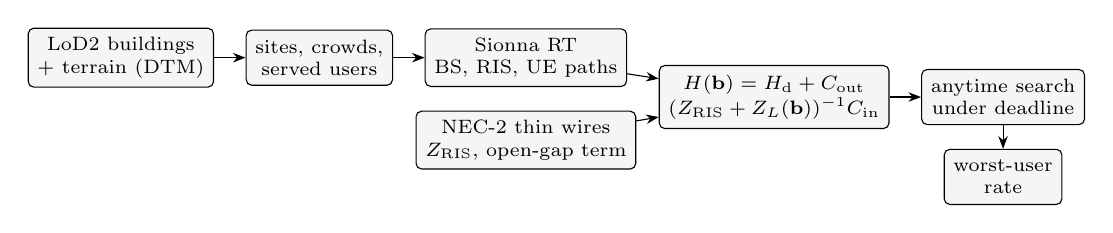
\begin{tikzpicture}[node distance=3mm and 4mm, every node/.style={font=\scriptsize}, box/.style={draw, rounded corners=2pt, align=center, minimum height=7mm, fill=gray!8}, >={Stealth[length=1.6mm]}]
\node[box] (lod) {LoD2 buildings\\+ terrain (DTM)};
\node[box, right=of lod] (sites) {sites, crowds,\\served users};
\node[box, right=of sites] (rt) {Sionna RT\\BS, RIS, UE paths};
\node[box, below=of rt] (nec) {NEC-2 thin wires\\$Z_{\mathrm{RIS}}$, open-gap term};
\node[box, right=of rt, yshift=-5mm] (op) {$H(\mathbf b)=\Hd+C_{\mathrm{out}}$\\$(Z_{\mathrm{RIS}}+Z_L(\mathbf b))^{-1}C_{\mathrm{in}}$};
\node[box, right=of op] (srch) {anytime search\\under deadline};
\node[box, below=of srch] (rate) {worst-user\\rate};
\draw[->] (lod) -- (sites); \draw[->] (sites) -- (rt); \draw[->] (rt) -- (op); \draw[->] (nec) -- (op); \draw[->] (op) -- (srch); \draw[->] (srch) -- (rate);
\end{tikzpicture}}
\caption{GeoRIS-Bench pipeline. Geometry is converted to ray-traced port-to-port paths; the surface is a multiport NEC-2 model; the exact operator gives the channel for every binary state $\mathbf b$.}\label{fig:pipeline}
\end{figure}

\subsection{Scenes, sites and users}
The development maps are Munich (Bavarian LoD2 and DGM1~\cite{bavaria2025lod2}), Rotterdam and Maastricht (3DBAG LoD2.2~\cite{peters2022automated}, distributed as CityJSON~\cite{ledoux2019cityjson}, on AHN4 terrain~\cite{ahn4}). Two further cities are held out geographically and were never opened. Building surfaces receive simple material classes; terrain gaps under footprints are filled by a guarded interpolation that never extrapolates.

Sites are planned from geometry only. A RIS candidate is a facade point 3--30\,m above local ground; a BS candidate is a rooftop point or a 12\,m street mast. The natural scope requires a clear BS--RIS segment of \res{siteDminNat}--\res{siteDmaxNat}\,m and a coverage rule on street probes: the BS and the RIS each see at least 10\% of probes, and the RIS sees probes in the BS shadow. Pedestrian groups follow routes on the street graph with natural speeds and heights; 2--4 users are served per clip. Each served slot is drawn from users with RIS line of sight (LOS), except that a slot is taken from users without it with probability \res{negSlotProb}, as declared negative cases. No user distance is used to accept or reject a case.

The natural scope has \res{prodTrajPerMap} trajectories per map, \res{prodFramesPerTraj} frames each (\res{prodFrames} frames, \res{prodArrayFrames} array-frames over three arrays). Splits are by trajectory: 70\% train, 15\% validation (\res{prodValTraj} trajectories) and 15\% test; the test part stays sealed in this paper, and all natural-scope numbers below come from validation only.

\subsection{Coupled channel operator}
Paths are traced at \res{freqGHz}\,GHz with Sionna RT~\cite{hoydis2023sionna} (maximum interaction depth \res{rtDepth}, specular reflection and diffraction enabled, \res{rtSamples} samples per source) between explicit port positions: four vertically polarised BS ports spaced by half a wavelength, every RIS element centre, and the served users. The surface is a lattice of $8\times8$, $8\times16$ or $16\times16$ thin vertical wires (24\,mm long, 50\,$\mu$m radius, 28/30\,mm pitch; panel sizes \res{natApW64}$\times$\res{natApH64}, \res{natApW128}$\times$\res{natApH128} and \res{natApW256}$\times$\res{natApH256}\,m), whose full impedance matrix $Z_{\mathrm{RIS}}$ is solved once with NEC-2~\cite{burke1981nec,pynec}. Every wire ends in one of two passive loads with 1\,$\Omega$ resistance and reactances $\pm70\,\Omega$ around the isolated-wire resonance. Reducing the port network by a Schur complement over the external ports, with 50\,$\Omega$ references, gives the end-to-end channel
\begin{equation}
H(\mathbf b)=\Hd + C_{\mathrm{out}}\bigl(Z_{\mathrm{RIS}}+Z_L(\mathbf b)\bigr)^{-1}C_{\mathrm{in}},\qquad Z_L(\mathbf b)=\mathrm{diag}\bigl(z_{b_1},\dots,z_{b_N}\bigr),
\label{eq:operator}
\end{equation}
where $C_{\mathrm{in}}$ maps the ray-traced incident field onto open-circuit element voltages through the embedded effective lengths and $C_{\mathrm{out}}$ maps element currents to the users by reciprocity. The open-gap wires scatter even when unloaded; this structural term changed a reference direct channel by \res{openGapPct}\% and is carried explicitly into $\Hd$. The panel is not part of the ray-traced mesh, so no RIS interaction is counted twice. Because $Z_L$ is diagonal, flipping one or two elements is a rank-one or rank-two update of the inverse in~\eqref{eq:operator}; Sherman--Morrison--Woodbury updates score all single and pair moves without a full re-solve, and every search method uses the same evaluator.

\subsection{Objective}
The served users' rates are computed under a regularised zero-forcing (RZF) precoder $W$ that is derived once per frame from the all-OFF channel, normalised to 0.1\,W, and then kept fixed for every candidate state. For user $k$,
\begin{equation}
\mathrm{SINR}_k(\mathbf b)=\frac{|[H(\mathbf b)W]_{kk}|^2}{\sum_{j\neq k}|[H(\mathbf b)W]_{kj}|^2+\sigma^2},
\end{equation}
and the objective is the worst-user rate $f(\mathbf b)=\min_k\log_2(1+\mathrm{SINR}_k(\mathbf b))$, with thermal noise over 1\,MHz and a 7\,dB noise figure. The task is $\max_{\mathbf b\in\{0,1\}^N} f(\mathbf b)$.

\subsection{Configuration methods}
All methods are anytime controllers: they start from the all-OFF state, keep the best state found, and must return by an absolute deadline that covers set-up, every scan and a final full rescore.
\textbf{No RIS} uses $\Hd$ only, and \textbf{all OFF} is the reference state. \textbf{Greedy} applies the best improving single flip until none improves and then restarts from a uniform random state. \textbf{Pair} does the same but, at a single-flip optimum, scans all $\binom N2$ pair flips before restarting (a 2-opt basin). \textbf{b3} replaces uniform restarts by restart densities alternating between $18/64$ and $0.5$; \textbf{b5} keeps up to eight distinct local optima and, every third restart, starts from a child that inherits each bit from one of two elites; \bthreefive{} combines both. \textbf{ME-GA} is our reimplementation of the memory-enhanced evolutionary controller of~\cite{zardi2024memory} from its published description, under the same deadline. Because the paper publishes no code or operator details, ME-GA is a specification-based baseline, not a reproduction.

%======================================================================
\section{Natural Scope: A Small Facade RIS Barely Matters}\label{sec:natural}
%======================================================================
For each of the \res{natFramesTotal} validation array-frames (\res{natTraj64} trajectories $\times$ 16 frames $\times$ 3 arrays) we computed the worst-user rate with no RIS, at all OFF, at all ON, and at the best state found by \bthreefive{} with a long deadline (300/500/800\,ms for 64/128/256 elements, never below all OFF). We also computed the precoder-free channel power of each user through the BS paths and through the RIS. Table~\ref{tab:natural} and Fig.~\ref{fig:natural} summarise the results.

\begin{table}[t]
\centering
\caption{Natural-scope leverage, validation split. Rates in bit/s/Hz; ``non-zero'' excludes frames whose all-OFF worst-user rate is zero. Power ratios are medians over users of the given BS/RIS visibility class, at the best state.}\label{tab:natural}
\footnotesize\setlength{\tabcolsep}{2.5pt}
\begin{tabular}{@{}lrrr@{}}
\toprule
Array size (elements) & 64 & 128 & 256\\
\midrule
Frames at worst-user rate 0 (all OFF) & \res{natZeroShare64}\% & \res{natZeroShare128}\% & \res{natZeroShare256}\%\\
\quad of which a served user has no path & \res{natZeroBoth64} & \res{natZeroBoth128} & \res{natZeroBoth256}\\
Trajectories at 0 in all frames (of \res{natTraj64}) & \res{natZeroTraj64} & \res{natZeroTraj128} & \res{natZeroTraj256}\\
All OFF $-$ no RIS, mean & \res{natOffMinusNoRis64} & \res{natOffMinusNoRis128} & \res{natOffMinusNoRis256}\\
Best $-$ all OFF, all frames, mean & \res{natGainAllMean64} & \res{natGainAllMean128} & \res{natGainAllMean256}\\
Best $-$ all OFF, non-zero frames, mean & \res{natGainNzMean64} & \res{natGainNzMean128} & \res{natGainNzMean256}\\
\quad median / 90th percentile & \res{natGainNzMedian64} / \res{natGainNzPninety64} & \res{natGainNzMedian128} / \res{natGainNzPninety128} & \res{natGainNzMedian256} / \res{natGainNzPninety256}\\
Frames with gain $>0.1$ / $>0.5$ & \res{natGainGtOne64} / \res{natGainGtFive64}\% & \res{natGainGtOne128} / \res{natGainGtFive128}\% & \res{natGainGtOne256} / \res{natGainGtFive256}\%\\
\midrule
RIS $-$ direct, BS blk./RIS LOS (dB) & \res{natRisDirBlkLos64} & \res{natRisDirBlkLos128} & \res{natRisDirBlkLos256}\\
RIS $-$ direct, BS refl./RIS LOS (dB) & \res{natRisDirRefLos64} & \res{natRisDirRefLos128} & \res{natRisDirRefLos256}\\
RIS $-$ direct, BS LOS/RIS LOS (dB) & \res{natRisDirLosLos64} & \res{natRisDirLosLos128} & \res{natRisDirLosLos256}\\
Ideal plate vs LOS, BS blk./RIS LOS (dB) & \res{natBoundBlkLos64} & \res{natBoundBlkLos128} & \res{natBoundBlkLos256}\\
\bottomrule
\end{tabular}
\end{table}

\begin{figure}[t]
\centering
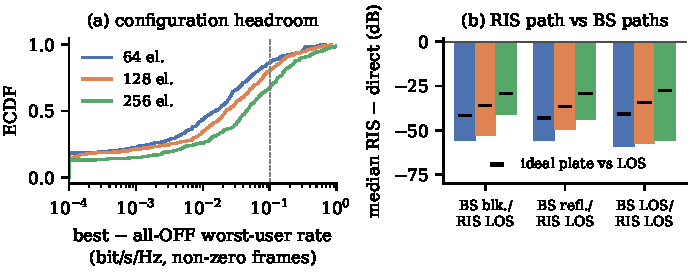
\includegraphics[width=\textwidth]{figures/natural_leverage.pdf}
\caption{Natural scope, validation. (a) Distribution of the configuration headroom on non-zero frames (values below $10^{-4}$ drawn at $10^{-4}$; dashed line at 0.1\,bit/s/Hz). (b) Median RIS-path minus BS-path power per user class at the best state, with the ideal-plate bound relative to a LOS path (black ticks).}\label{fig:natural}
\end{figure}

\textbf{Half of the frames are degenerate.} In \res{natZeroShare64}\% of the 64-element frames the worst-user rate is exactly zero, and in \res{natZeroBoth64} of the \res{natFrames64} frames the cause is that one served user has neither a direct nor a RIS channel: the tracer, with two interactions and diffraction, finds no path to a user blocked from both the BS and the surface. \res{natZeroTraj64} of \res{natTraj64} validation trajectories are at zero in all frames. The share depends strongly on the city (\res{natZeroMaastricht64}\% Maastricht, \res{natZeroMunich64}\% Munich, \res{natZeroRotterdam64}\% Rotterdam at 64 elements). These users enter through the declared negative slots and through the fallback when no RIS-reachable user exists; the scheduler does not require a served user to have any path. On such frames every method returns zero, so any comparison of methods is an exact tie.

\textbf{Where users are reachable, the headroom is small.} Adding the surface in its all-OFF state raises the mean worst-user rate by \res{natOffMinusNoRis64}, \res{natOffMinusNoRis128} and \res{natOffMinusNoRis256}\,bit/s/Hz at 64, 128 and 256 elements. Configuring it helps little more: on non-zero frames the median gain of the long-deadline search over all OFF is \res{natGainNzMedian64}, \res{natGainNzMedian128} and \res{natGainNzMedian256}\,bit/s/Hz, and only \res{natGainGtOne64}\%, \res{natGainGtOne128}\% and \res{natGainGtOne256}\% of frames gain more than 0.1. The headroom grows with array size, as coherent aperture gain predicts, but remains far below the differences that separate search algorithms in Sect.~\ref{sec:freespace}. It concentrates where the worst user sees both the BS and the RIS: at 256 elements, \res{natHrNLosLos256} such frames have a median gain of \res{natHrMedLosLos256} (\res{natHrGtLosLos256}\% above 0.1), against \res{natHrMedBlkLos256} for \res{natHrNBlkLos256} frames whose worst user is BS-blocked.

\textbf{Cause: the RIS path is 40--60\,dB weaker than the BS paths.} At the best state, the median RIS-path power of a BS-blocked user with RIS LOS is \res{natRisDirBlkLos64}, \res{natRisDirBlkLos128} and \res{natRisDirBlkLos256}\,dB relative to that user's BS paths (Table~\ref{tab:natural}). A user that is blocked from the BS still receives reflected or diffracted BS paths that are much stronger than the re-radiation of a panel \res{natApW64}--\res{natApW256}\,m wide at a median \res{natDbsrisMedian}\,m from the BS (maximum \res{natDbsrisMax}\,m), with median RIS--user distances of \res{natDrisUserLo}--\res{natDrisUserHi}\,m. No validation frame contains a user served only through the RIS; the only class in which the RIS path is stronger (BS blocked, RIS reflection only; \res{natUFBlkRef64} user-frames from one trajectory) is negligible.

\textbf{The gap is physical, not a modelling artefact.} An ideal, lossless plate of aperture $A$, perfectly steered, re-radiates to a user at distance $d_2$ from a BS at distance $d_1$ with power relative to a LOS path of length $d$ bounded by
\begin{equation}
\frac{P_{\mathrm{RIS}}}{P_{\mathrm{LOS}}}\le\frac{A^2d^2}{\lambda^2d_1^2d_2^2},
\label{eq:bound}
\end{equation}
with $\lambda=\res{lambdaMm}$\,mm. Evaluated on the actual geometry, the bound places even an ideal plate \res{natBoundBlkLos64}\,dB (64 elements) to \res{natBoundBlkLos256}\,dB (256 elements) below LOS for BS-blocked users (Fig.~\ref{fig:natural}b). The 1-bit coupled array cannot reach this bound, and a BS-blocked user still has reflected and diffracted BS paths, so the realised RIS-to-direct ratios in Table~\ref{tab:natural} are lower still.

\textbf{Ruled out.} The stored precoder equals the RZF of the all-OFF channel (maximum relative error \res{natPrecErr64}); re-deriving the RZF for the best state does not raise the rate (mean \res{natRateBestOwnMean64} against \res{natRateBestMean64} at 64 elements). Interference is below noise for the worst user (median interference-to-noise ratio \res{natIN64}, \res{natIN128} and \res{natIN256}\,dB). Transmit power scales both paths equally and cannot change their ratio.

The natural scope therefore supports a clear finding for deployment: \emph{a small facade RIS around one hundred metres from the BS barely changes the worst-user rate in LoD2 cities.} It also shows that this scope cannot rank configuration algorithms, since about half the frames are exact ties and the rest offer a median headroom of a few hundredths of a bit/s/Hz.

%======================================================================
\section{RIS-Relevant Scope}\label{sec:relevant}
%======================================================================
Bound~\eqref{eq:bound} indicates where the surface can matter. For a BS-blocked user, $d\approx d_2$ and the ratio scales as $(A/\lambda d_1)^2$; a 256-element panel reaches $-10$\,dB of LOS when $d_1d_2/d\approx\res{boundXtenDb}$\,m. Moving the BS--RIS distance from the natural median of 112\,m to at most 20\,m raises the RIS-to-direct ratio by at least \res{rrShiftDb}\,dB. We therefore declared, before generating any geometry, a RIS-relevant scope with three changes:
\begin{itemize}
\item \textbf{Sites:} the natural site procedure with the BS--RIS distance restricted to \res{rrDmin}--\res{rrDmax}\,m (fallback \res{rrDmin}--\res{rrDmaxFallback}\,m if too few sites exist).
\item \textbf{Crowds:} each group anchor is moved, with probability \res{rrAnchorProb}, into the zone of street probes that the RIS sees and the BS does not.
\item \textbf{Served users:} only users that are BS-blocked and RIS-LOS in every selected frame are eligible; there are no negative slots and no fallback. After tracing, frames with a pathless served user are flagged and excluded.
\end{itemize}
All rules use geometry labels only, never rates. The pilot uses one map (\res{rrMap}), \res{rrTraj} trajectories (\res{rrFrames} frames, \res{rrArrayFrames} array-frames), split into \res{rrTrainTraj} training, \res{rrValTraj} validation and \res{rrTestTraj} sealed test trajectories, with a new seed stream disjoint from all earlier draws. A leverage gate, fixed in advance and evaluated on validation only, decides whether the scope is promoted to a benchmark (Table~\ref{tab:gate}). Its thresholds take a conservative 10\,dB of the predicted shift, i.e.\ a factor $\sqrt{10}$ on the natural-scope gains.

\begin{table}[t]
\centering
\caption{Declared leverage gate of the RIS-relevant pilot (validation, unflagged frames) and observed values. Red P: pending the pilot run (macros \texttt{rr*} in \texttt{results.tex}).}\label{tab:gate}
\pendshorttrue\footnotesize\setlength{\tabcolsep}{4pt}
\begin{tabular}{@{}llrrr@{}}
\toprule
Gate & Quantity & 64 & 128 & 256\\
\midrule
L1a & pathless served user-frames ($\le$\res{rrLoneA}\%) & \res{rrLoneAobs64} & \res{rrLoneAobs128} & \res{rrLoneAobs256}\\
L1b & flagged frames ($\le$\res{rrLoneB}\%; natural \res{natZeroShare64}\%) & \res{rrLoneBobs64} & \res{rrLoneBobs128} & \res{rrLoneBobs256}\\
L2 & median best $-$ all OFF, threshold & $\ge$\res{rrLtwo64} & $\ge$\res{rrLtwo128} & $\ge$\res{rrLtwo256}\\
 & \quad observed & \res{rrGainMedian64} & \res{rrGainMedian128} & \res{rrGainMedian256}\\
L3 & median all OFF $-$ no RIS, threshold & $\ge$\res{rrLthree64} & $\ge$\res{rrLthree128} & $\ge$\res{rrLthree256}\\
 & \quad observed & \res{rrOffMinusNoRis64} & \res{rrOffMinusNoRis128} & \res{rrOffMinusNoRis256}\\
-- & frames with gain $>0.1$ (reported) & \res{rrGainGtOne64} & \res{rrGainGtOne128} & \res{rrGainGtOne256}\\
-- & median RIS $-$ direct, dB (reported) & \res{rrRisDir64} & \res{rrRisDir128} & \res{rrRisDir256}\\
\midrule
\multicolumn{2}{@{}l}{Gate verdict} & \multicolumn{3}{c}{\res{rrGate}}\\
\bottomrule
\end{tabular}
\end{table}

\textbf{Array size and coupling.} On this scope we report how the headroom grows from 64 to 256 elements (Table~\ref{tab:gate}) and the effect of coupling. For the latter, a coupling-blind search uses only the diagonal of $Z_{\mathrm{RIS}}$ in its internal model, and every state it returns is rescored on the full operator~\eqref{eq:operator}. The rate-prediction error of the diagonal model is \res{rrCoupMae64}, \res{rrCoupMae128} and \res{rrCoupMae256}\,bit/s/Hz and the rate lost by its chosen states is \res{rrCoupLoss64}, \res{rrCoupLoss128} and \res{rrCoupLoss256}\,bit/s/Hz at 64, 128 and 256 elements. For reference, on one frame of the free-space geometry of Sect.~\ref{sec:freespace}, removing inter-element coupling changed the predicted rate by \res{fsCoupMae}\,bit/s/Hz in mean absolute terms over \res{fsCoupPatterns} random states, a development diagnostic rather than a held-out result.

\textbf{Method ranking.} Table~\ref{tab:rrmethods} ranks the methods of Sect.~\ref{sec:bench} at the 50\,ms deadline on the validation part. With \res{rrValTraj} validation trajectories, the ranking is descriptive; confirmatory contrasts would require the sealed part and a separate declaration.

\begin{table}[t]
\centering
\caption{RIS-relevant pilot, validation: mean worst-user rate (bit/s/Hz) at 50\,ms and two contrasts with trajectory-bootstrap intervals. Red P: pending the pilot run.}\label{tab:rrmethods}
\pendshorttrue\footnotesize\setlength{\tabcolsep}{3pt}
\begin{tabular}{@{}lrrrrrrrr@{}}
\toprule
Elements & no RIS & all OFF & greedy & pair & \bthreefive{} & ME-GA & \bthreefive{}$-$pair & pair$-$greedy\\
\midrule
64 & \res{rrRateNoRis64} & \res{rrRateAllOff64} & \res{rrRateGreedy64} & \res{rrRatePair64} & \res{rrRateBts64} & \res{rrRateMega64} & \res{rrDBtsPair64} & \res{rrDPairGreedy64}\\
128 & \res{rrRateNoRis128} & \res{rrRateAllOff128} & \res{rrRateGreedy128} & \res{rrRatePair128} & \res{rrRateBts128} & \res{rrRateMega128} & \res{rrDBtsPair128} & \res{rrDPairGreedy128}\\
256 & \res{rrRateNoRis256} & \res{rrRateAllOff256} & \res{rrRateGreedy256} & \res{rrRatePair256} & \res{rrRateBts256} & \res{rrRateMega256} & \res{rrDBtsPair256} & \res{rrDPairGreedy256}\\
\bottomrule
\end{tabular}
\end{table}

%======================================================================
\section{Controlled Physics: Free-Space Coupled Surface}\label{sec:freespace}
%======================================================================
To evaluate configuration algorithms where the surface certainly matters, we use a free-space reference in which BS, users and surface share one NEC-2 model: 64 wires as above, four BS wires and two user wires form a single 70-port structure, so that coupling between all antennas is retained. All ports lie in a sub-metre region around the panel, a deliberately surface-dominated geometry. Users move along straight trajectories of 16 frames at 20\,ms spacing. The production mesh has 81 segments per wire; every returned state is also rescored on an independent 161-segment mesh, and the 161-segment rate is the primary outcome.

\textbf{Protocol.} The protocol was frozen before the run: \res{fsTraj} held-out trajectories (\res{fsFrames} frames) never used for design, six methods, deadlines of 5, 10, 50 and 100\,ms, and \res{fsSeeds} seeds (\res{fsRunsPerCell} runs per method and deadline). The timed section, pinned to one CPU core with single-threaded numerical libraries, contains network set-up, all scans and the final rescore. The unit of analysis is the trajectory (frames and seeds averaged), with paired bootstrap intervals (\res{fsBoot} resamples) under a Bonferroni correction over five contrasts per deadline. A contrast is supported only if its interval excludes zero on both meshes and neither method misses more than \res{fsMaxMiss}\% of its deadlines. The \res{fsPrimary}\,ms deadline is confirmatory; the others are secondary. \bthreefive{} was selected on development trajectories from the same generator.

\begin{figure}[t]
\centering
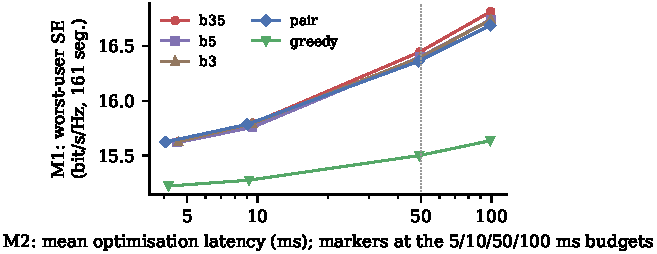
\includegraphics[width=0.62\textwidth]{figures/freespace_budget.pdf}
\caption{Free-space coupled reference, held-out test: mean worst-user rate against the full-runtime deadline (ME-GA, far below, omitted; see Table~\ref{tab:freespace}).}\label{fig:freespace}
\end{figure}

\begin{table}[t]
\centering
\caption{Free-space held-out test. Top: mean worst-user rate (bit/s/Hz, 161 segments). Bottom: confirmatory contrasts at 50\,ms with Bonferroni intervals on both meshes and trajectories won (of \res{fsN}).}\label{tab:freespace}
\footnotesize\setlength{\tabcolsep}{3pt}
\begin{tabular}{@{}lrrrrrr@{}}
\toprule
Deadline & greedy & pair & ME-GA & b3 & b5 & \bthreefive{}\\
\midrule
5\,ms & \res{fsRateGreedyFive} & \res{fsRatePairFive} & \res{fsRateMegaFive} & \res{fsRateBthreeFive} & \res{fsRateBfiveFive} & \res{fsRateBtsFive}\\
10\,ms & \res{fsRateGreedyTen} & \res{fsRatePairTen} & \res{fsRateMegaTen} & \res{fsRateBthreeTen} & \res{fsRateBfiveTen} & \res{fsRateBtsTen}\\
50\,ms & \res{fsRateGreedyFifty} & \res{fsRatePairFifty} & \res{fsRateMegaFifty} & \res{fsRateBthreeFifty} & \res{fsRateBfiveFifty} & \textbf{\res{fsRateBtsFifty}}\\
100\,ms & \res{fsRateGreedyHundred} & \res{fsRatePairHundred} & \res{fsRateMegaHundred}$^\dagger$ & \res{fsRateBthreeHundred} & \res{fsRateBfiveHundred} & \textbf{\res{fsRateBtsHundred}}\\
\midrule
\end{tabular}

\resizebox{\textwidth}{!}{\begin{tabular}{@{}lllrl@{}}
Contrast (50\,ms) & 161 segments & 81 segments & Won & Verdict\\
\midrule
\bthreefive{} $-$ pair & \res{fsDBtsPairFifty} [\res{fsLoBtsPairFifty}, \res{fsHiBtsPairFifty}] & \res{fsDEiBtsPairFifty} [\res{fsLoEiBtsPairFifty}, \res{fsHiEiBtsPairFifty}] & \res{fsWinsBtsPairFifty} & \res{fsSupBtsPairFifty}\\
\bthreefive{} $-$ b3 & \res{fsDBtsBthreeFifty} [\res{fsLoBtsBthreeFifty}, \res{fsHiBtsBthreeFifty}] & \res{fsDEiBtsBthreeFifty} [\res{fsLoEiBtsBthreeFifty}, \res{fsHiEiBtsBthreeFifty}] & \res{fsWinsBtsBthreeFifty} & \res{fsSupBtsBthreeFifty}\\
\bthreefive{} $-$ b5 & \res{fsDBtsBfiveFifty} [\res{fsLoBtsBfiveFifty}, \res{fsHiBtsBfiveFifty}] & \res{fsDEiBtsBfiveFifty} [\res{fsLoEiBtsBfiveFifty}, \res{fsHiEiBtsBfiveFifty}] & \res{fsWinsBtsBfiveFifty} & \res{fsSupBtsBfiveFifty}\\
\bthreefive{} $-$ ME-GA & \res{fsDBtsMegaFifty} [\res{fsLoBtsMegaFifty}, \res{fsHiBtsMegaFifty}] & \res{fsDEiBtsMegaFifty} [\res{fsLoEiBtsMegaFifty}, \res{fsHiEiBtsMegaFifty}] & \res{fsWinsBtsMegaFifty} & \res{fsSupBtsMegaFifty}\\
pair $-$ greedy & \res{fsDPairGreedyFifty} [\res{fsLoPairGreedyFifty}, \res{fsHiPairGreedyFifty}] & \res{fsDEiPairGreedyFifty} [\res{fsLoEiPairGreedyFifty}, \res{fsHiEiPairGreedyFifty}] & \res{fsWinsPairGreedyFifty} & \res{fsSupPairGreedyFifty}\\
\bottomrule
\end{tabular}}

\smallskip\scriptsize $^\dagger$ME-GA missed \res{fsMissMegaHundred} of \res{fsRunsPerCell} deadlines at 100\,ms (\res{fsMissPctMegaHundred}\%) and is excluded there; at 50\,ms it missed \res{fsMissMegaFifty}. All other methods missed none.
\end{table}

\textbf{Results.} All five confirmatory contrasts are supported (Table~\ref{tab:freespace}). At 50\,ms, \bthreefive{} exceeds exact pair search by \res{fsDBtsPairFifty}\,bit/s/Hz [\res{fsLoBtsPairFifty}, \res{fsHiBtsPairFifty}] and wins \res{fsWinsBtsPairFifty} of \res{fsN} trajectories; the estimate on the 81-segment mesh is \res{fsDEiBtsPairFifty}. It also beats each of its components, so restart densities and elite recombination both contribute. Pair moves matter more than either: pair search exceeds greedy single-flip search by \res{fsDPairGreedyFifty}\,bit/s/Hz. Fig.~\ref{fig:freespace} shows that the advantage of \bthreefive{} needs time: at 5\,ms (\res{fsDBtsPairFive} [\res{fsLoBtsPairFive}, \res{fsHiBtsPairFive}]) and 10\,ms (\res{fsDBtsPairTen}) the contrast with pair is not supported, because only a few restarts fit into the deadline, while at 100\,ms it grows to \res{fsDBtsPairHundred} [\res{fsLoBtsPairHundred}, \res{fsHiBtsPairHundred}]. The specification-based ME-GA reaches \res{fsRateMegaFifty}\,bit/s/Hz at 50\,ms, well below every local-search method; as declared before the run, this contrast measures distance to a published specification, not a contest between tuned methods. Mesh shifts at 50\,ms are small and similar across the pair-based methods (\res{fsShiftPairFifty} for pair, \res{fsShiftBtsFifty} for \bthreefive{}), so the contrasts barely move between meshes.

In this geometry the configuration changes the worst-user rate by bit/s/Hz rather than hundredths of one, and search quality under a deadline separates methods clearly. This is the regime that the natural city scope does not reach.

%======================================================================
\section{Discussion: When Does Configuration Matter?}\label{sec:discussion}
%======================================================================
Read together, the three settings separate two questions. \emph{Does configuration matter?} depends on the power ratio between the surface path and the BS paths, which is set by aperture, wavelength and the product of the two hop distances~\eqref{eq:bound}, and on whether the served users have any path at all. In the natural scope both conditions fail for most frames. In the free-space reference both hold. The RIS-relevant scope is designed to sit between them, and its gate turns the bound into a falsifiable prediction. \emph{Which algorithm configures best?} can be answered only where the first answer is yes; in the free-space regime the answer is a pair-move local search with structured restarts, and the margin over simpler search depends on the deadline.

Three practical lessons follow for data-driven RIS research. First, a benchmark should report its \emph{leverage} -- the distribution of best-minus-reference gain and the share of degenerate frames -- before any method comparison; otherwise null results are uninterpretable. Second, served-user rules must guarantee a traced path, since a pathless user turns the max--min objective into a constant. Third, deadlines should cover the complete controller, including set-up and final rescoring; at short deadlines the more elaborate search loses its advantage.

\textbf{Limitations.} The city channels rely on LoD2 geometry with simple materials, two ray interactions and no vegetation or vehicles; full-wave accuracy at city scale and measured hardware are outside our claims. The wire surface omits substrate, ground plane and switch parasitics. The 256-element model uses one mesh only, and the 161-segment free-space mesh is a consistency check rather than a convergence proof. Precoding uses the all-OFF channel throughout. The free-space test covers one geometry and one distribution, and the RIS-relevant pilot covers one map.

%======================================================================
\section{Conclusion}
%======================================================================
We combined open city models, ray tracing and an exact coupled multiport surface model into GeoRIS-Bench and asked when 1-bit RIS configuration matters. A small facade surface around a hundred metres from the BS barely changes the worst-user rate in three LoD2 cities: half the frames have a pathless user, and elsewhere the surface path is 40--60\,dB below the BS paths, consistent with an ideal-plate bound. Where the surface dominates, configuration matters and algorithms separate clearly: under a 50\,ms full-runtime deadline, pair search with structured restarts and elite recombination beats exact pair search on a frozen held-out test. A RIS-relevant scope, declared from the bound before tracing, connects the two regimes and will provide the benchmark on which array size, coupling and learned controllers can be compared meaningfully.

\subsubsection*{Disclosure of Interests.} The authors have no competing interests to declare that are relevant to the content of this article.

\bibliographystyle{splncs04}
\bibliography{references}
\end{document}
